\subsection{Analytic Evaluation (AE)}
\label{sec:Ana}

Performance analysis in context of DS-DSE is concerned about overall trends. Hence, the finer grained scheduling details of a TLM simulation are less important. As \ga targets streaming applications, the steady state performance is most important. 

The kernels in a streaming application operate as producers / consumers over the streaming data creating a pipeline. \figref{fig:Pipe} visualizes the pipeline execution for two HWACCs and one SW core. Each stage overlaps communication (in/out) with processing due to double buffering. Actors execute concurrently given their dependencies across different components. Actors mapped to the same component execute sequentially (e.g. in \emph{S8}).

\newtext{Our Analytic Evaluation (AE) model} computes the throughput of an application based on the inter-kernel pipelined execution~\cite{Teimouri_DAC_2015}.
At this abstraction, the throughput only depends on the pipe latency which is determined by the slowest processing component (or communication).

\begin{figure}[h]
	%\vspace{-10pt}
	\centering
	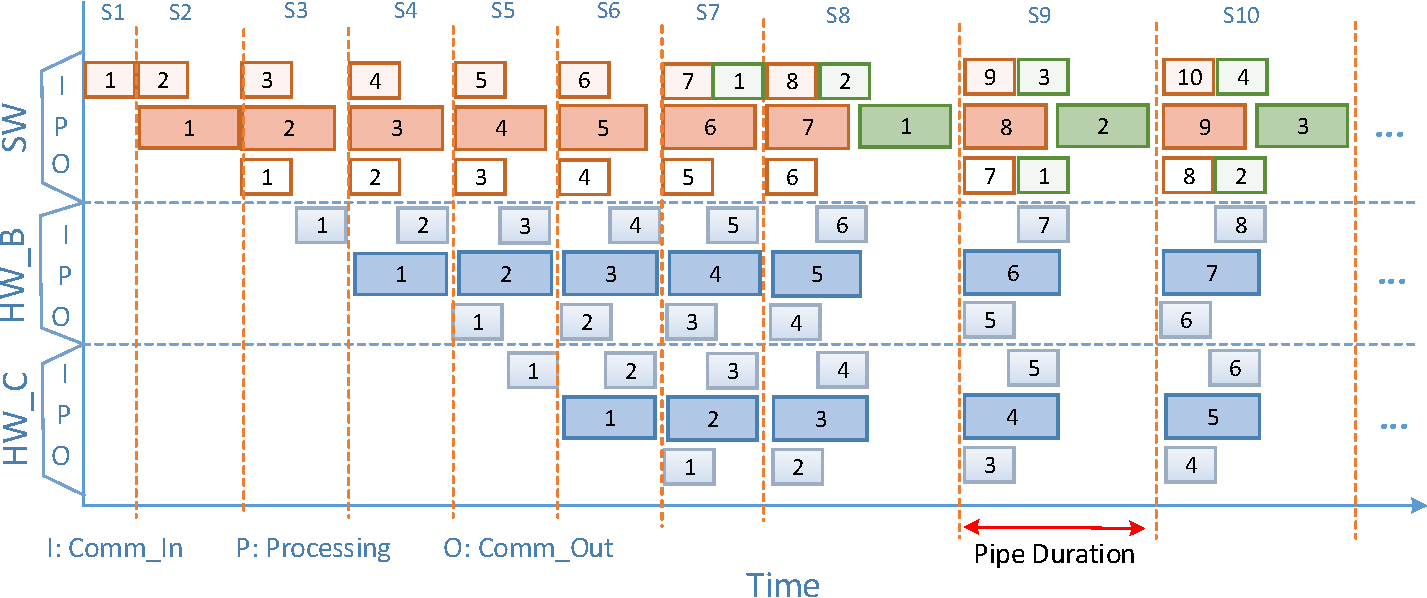
\includegraphics[width=\linewidth]{fig/pPipe.pdf}
	%\vspace{-10pt}
	\caption{Timing diagram of Architecture}
	\label{fig:Pipe}
	%\vspace{-6pt}
	
\end{figure}


Eq.~\eqref{eq:pipe} symbolically summarizes the AE model. The estimated throughput is equal to output volume per iteration $D_{C}(out)$ over the pipe latency $L_{Pipe}$. \newtext{$L_{Pipe}$ is the maximum latency of SW ($L_{SW_i}$), HW ($L_{HW_j}$), and each layer of communication fabric ($L_{CE_k}$). }

\begin{equation}
\begin{split}
	&Throughput = D_{C}(out) / L_{Pipe} \\
	&L_{Pipe} = Max (\forall L_{SW}, \forall L_{HW}, \forall L_{CE}) \\
	&L_{SW_i} = \frac{\sum_{T \in SW_i} D_{P}(T)} {Freq_{SW}} + L_{sync} \\
	&L_{HW_j} = \frac{\sum_{T \in HW_j} D_{P}(T)} {Freq_{SW}*20} \\
	&L_{CE_k} = \frac{\sum_{C \in CE_k} D_{C}} {BW_{CE} * Freq_{CE}}
\label{eq:pipe}
\end{split}
\end{equation}

 \newtext{SW latency $L_{SW_i}$} is the accumulation of processing (i.e. total SW processing demand) and synchronization $L_{sync}$. Synchronization $L_{sync}$ is due to coordinating HW/SW communication including interrupt requests (from DMA, HW).
\newtext{HW latency $L_{HW_j}$} is due to processing an actor in HW. Each HWACC only executes one function type. 
The processing acceleration of an ACC depends on its frequency and the parallelism of the FT implemented on the ACC. For simplicity and clarity of explanation, this paper assumes a uniform HW acceleration of 20x. Non-uniform acceleration can be considered by defining an acceleration per function type.
\newtext{Communication latency $L_{CE_k}$} depends on the communication volume (between SW and HW) over bandwidth. Hence contention is only considered as an average. A multi-layer communication fabric is assumed. 